\documentclass{article}

\usepackage{graphicx}
\usepackage{tikz}
\usepackage{tikzsymbols}
\usetikzlibrary{calc,patterns,shapes.geometric}
\pagestyle{empty}
\usepackage[margin=0pt]{geometry}
\geometry{papersize={14in,12in}}

\def\centerarc[#1](#2)(#3:#4:#5){\draw[#1] ($(#2)+({#5*cos(#3)},{#5*sin(#3)})$) arc (#3:#4:#5);}

\begin{document}
	\begin{figure}
		\centering
		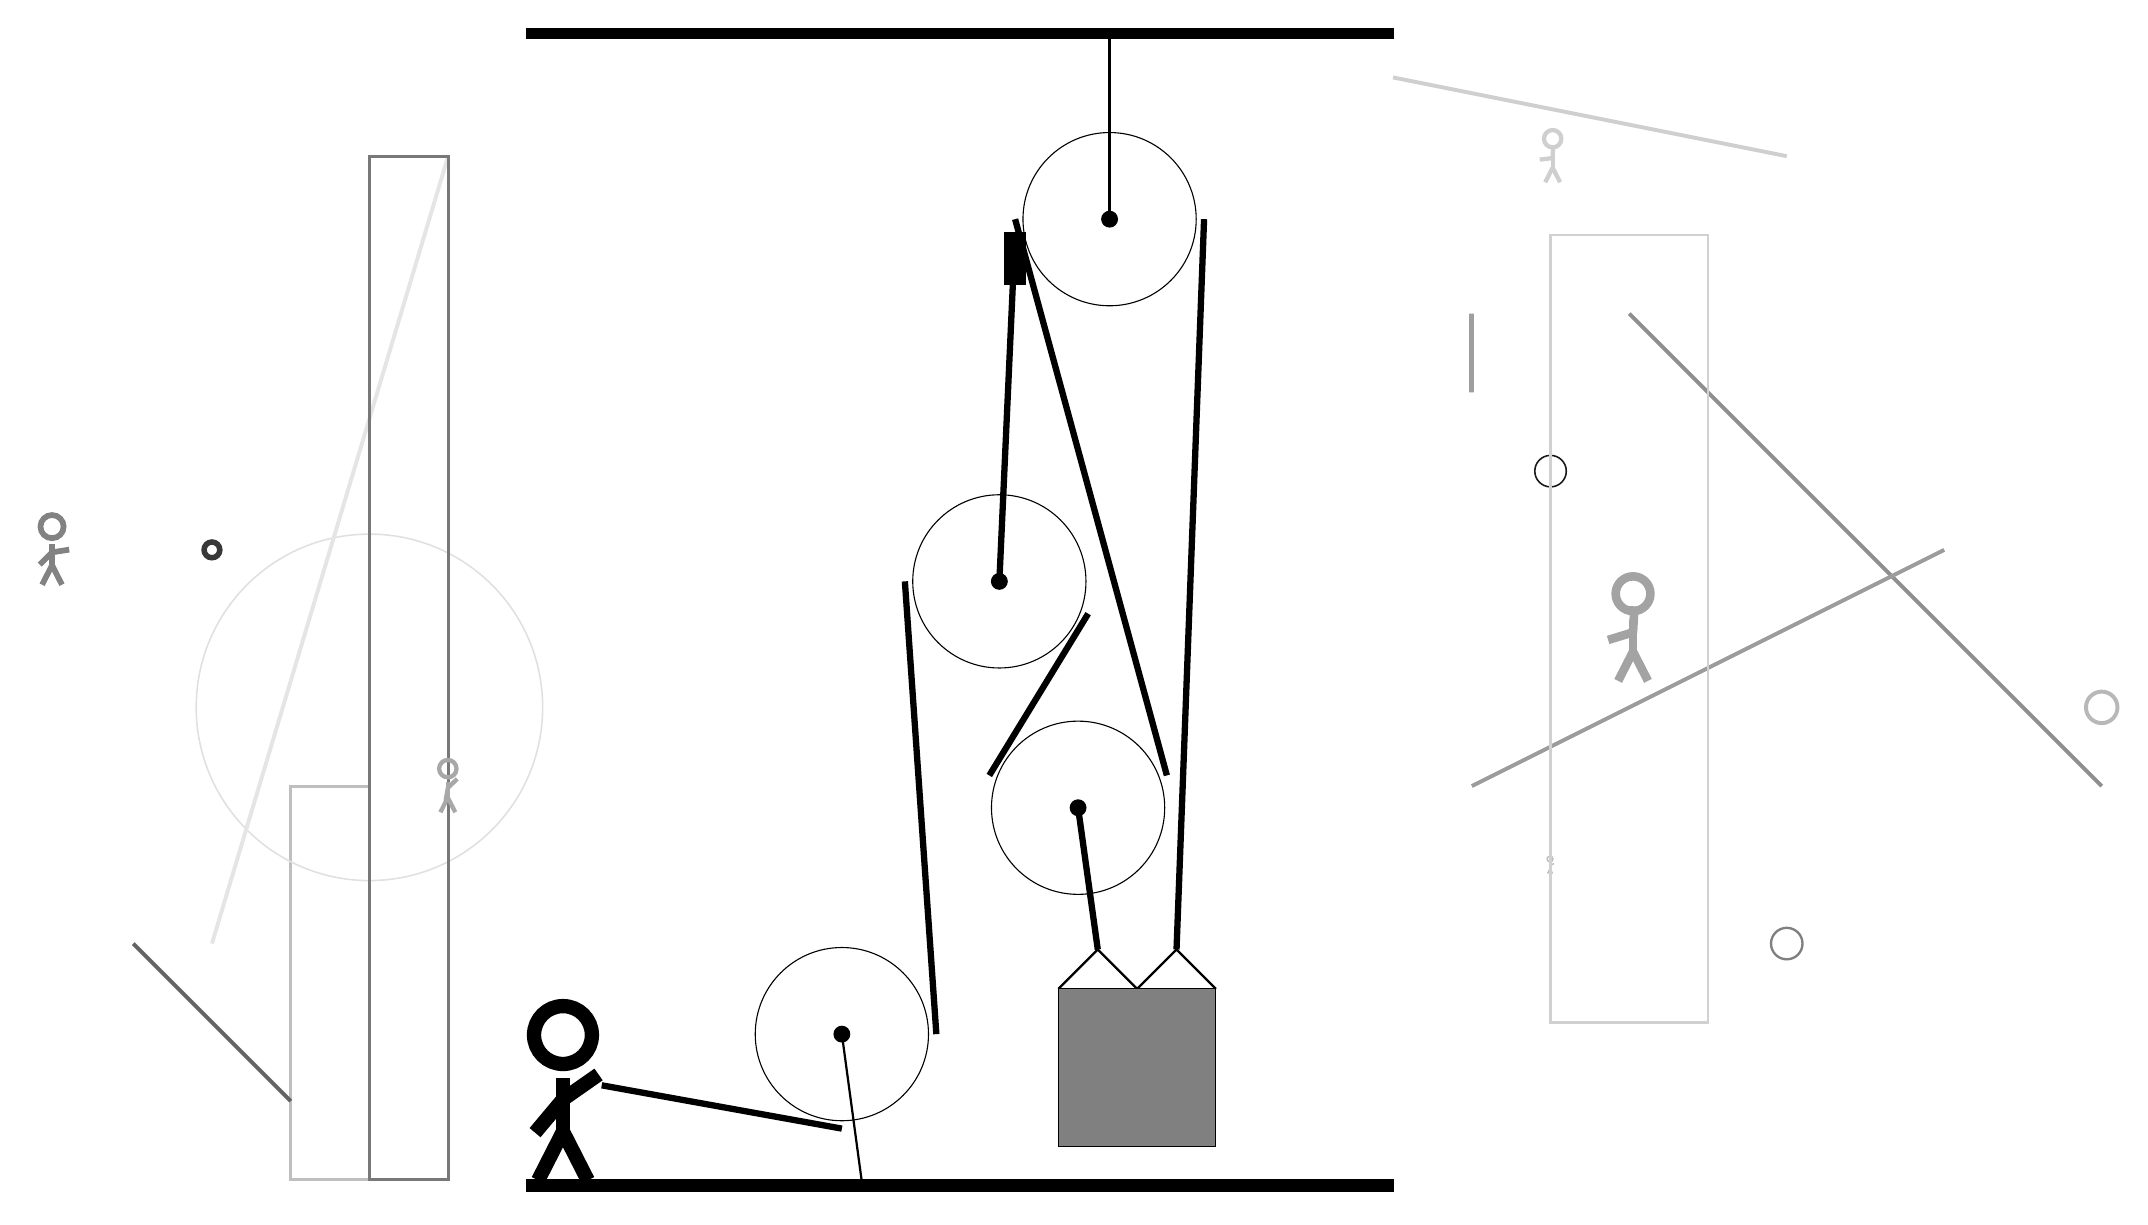
\begin{tikzpicture}
			%%%%% START %%%%%
			
			\draw[fill=black] (-6, 11.5) rectangle (5, 11.625);
			
			\draw (0, 4.6) circle (1.1);
			\draw[fill=black] (0, 4.6) circle (0.1);
			
			\draw (1, 1.725) circle (1.1);
			\draw[fill=black] (1, 1.725) circle (0.1);
			
			\draw[line width=0.4mm, color=black!25] (-8, -3) rectangle (-9, 2);
			
			\draw [line width=0.2mm, color=black!12](-8, 3) circle (2.2);
			\node[line width=0.2mm, color=black!19] at (7, 10) {\Strichmaxerl[3][7][88]};
			\node[line width=0.6mm, color=black!26] at (7, 1) {\Strichmaxerl[1][89][26]};
			
			\draw[line width=0.5mm, color=black!19](10, 10) -- (5, 11);
			
			\draw [line width=0.3mm, color=black!50](10, 0) circle (0.2);
			\draw[line width=0.5mm, color=black!10](-10, 0) -- (-7, 10);
			
			\draw [line width=0.6mm, color=black!62](7, 2) circle (0.0);
			\draw [line width=0.2mm, color=black!90](7, 6) circle (0.2);
			\draw[line width=0.5mm, color=black!44](8, 8) -- (14, 2);
			\draw [line width=0.5mm, color=black!28](14, 3) circle (0.2);
			\draw[line width=0.4mm, color=black!53] (-7, 10) rectangle (-8, -3);
			\draw [line width=0.7mm, color=black!78](-10, 5) circle (0.1);
			\draw[line width=0.5mm, color=black!61](-11, 0) -- (-9, -2);
			\draw[line width=0.5mm, color=black!39](6, 2) -- (12, 5);
			\draw[line width=0.3mm, color=black!18] (7, 9) rectangle (9, -1);
			
			\draw[line width=0.6mm, color=black!38] (6, 7) rectangle (6, 8);
			\node[line width=0.5mm, color=black!34] at (-7, 2) {\Strichmaxerl[3][80][44]};
			\node[line width=0.4mm, color=black!49] at (-12, 5) {\Strichmaxerl[4][45][9]};
			\node[line width=0.6mm, color=black!36] at (8, 4) {\Strichmaxerl[6][17][87]};
			
			\draw (1.4, 9.2) circle (1.1);
			\draw[fill=black] (1.4, 9.2) circle (0.1);
			\draw[very thick] (1.4, 9.2) -- (1.4, 11.5);
			
			\draw (-2, -1.15) circle (1.1);
			\draw[fill=black] (-2, -1.15) circle (0.1);
			\draw[thick] (-2, -1.15) -- (-1.75, -3);
			
			
			\draw[thick]  (0.75, -0.575) -- (1.25, -0.075) -- (1.75, -0.575) -- (2.25, -0.075) -- (2.75, -0.575);
			\draw[fill=black!50] (0.75, -0.575) rectangle (2.75, -2.575);
			\draw[line width=0.8mm] (-5.05, -1.8) -- (-2, -2.35);
			\centerarc[line width=0.8mm](-2, -1.15)(270:360:1.2000000000000002);
			\draw[line width=0.8mm] (-0.8, -1.15) -- (-1.2, 4.6);
			\draw[line width=0.8mm] (0, 4.6) -- (0.2, 9.0);
			\draw[line width=0.8mm, fill=black](0.1, 8.4) rectangle (0.3, 9.0);
			\centerarc[line width=0.8mm](0, 4.6)(-20:180:1.2000000000000002);
			\draw[line width=0.8mm] (1.1276, 4.1896) -- (-0.1276, 2.1354);
			\centerarc[line width=0.8mm](1, 1.725)(160:380:1.2000000000000002);
			\draw[line width=0.8mm] (2.1276, 2.1354) -- (0.2, 9.2);
			\draw[line width=0.8mm](1, 1.725) -- (1.25, -0.075);
			\centerarc[line width=0.8mm](1.4, 9.2)(0:180:1.2000000000000002);
			\draw[line width=0.8mm] (2.6, 9.2) -- (2.25, -0.075);
			
			\node at (-5.5, -1.9) {\Strichmaxerl[10][50][35]};
			
			\draw[fill=black] (-6, -3) rectangle (5, -3.15);
			
			%%%%% END %%%%%
		\end{tikzpicture}
	\end{figure}	
\end{document}